%!TEX root = ./slides_present.tex

\begin{frame}[plain]
\titlepage
\note{The Yang Lab is interested in developing statistical and computational methods/tools for quantitative genomics data analysis and biomedical data analysis}
\end{frame}


\begin{frame}
\frametitle{Table of Contents}
\tableofcontents
\end{frame}




\section{Background: GWAS, TWAS, \& PWAS}


\begin{frame}[fragile]{Central Dogma of Molecular Biology}
% \begin{columns}
%   \begin{column}{.4\textwidth}
    \begin{figure}
    \vspace*{-0.3cm}  
      \hspace*{-0.65cm}  
      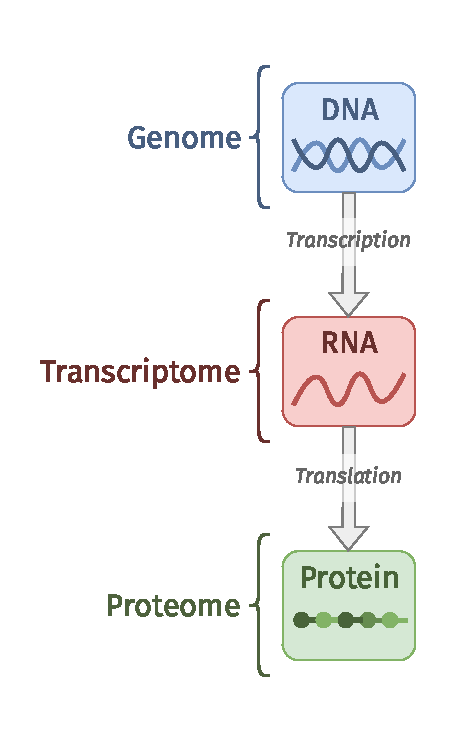
\includegraphics[width=0.5\textwidth]{../drawio_figs/bio_bg_2-1.drawio.pdf}
    \end{figure}
\note{ 
  expression DNA code is turned into a functional product\\
  in typical datasets we have:
  ~10mil variants \\
  ~20k RNA transcripts \\
  ~10k proteins
}
\end{frame}


\begin{frame}[fragile]{Genome-Wide Association Studies (GWAS)}
\begin{columns}
  \begin{column}[T]{.3\textwidth}
    \begin{figure}%
      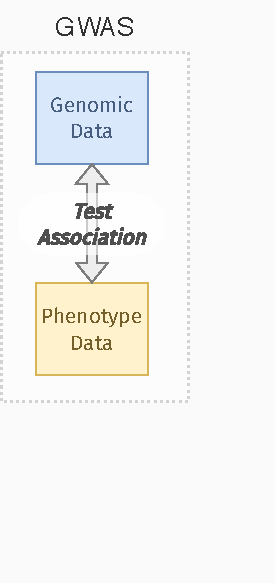
\includegraphics[width=14em]{../drawio_figs/bio_bg_2-GWAS_2bg.pdf}
    \end{figure}
  \end{column}
  %\hfill
  \begin{column}[T]{.7\textwidth}
   % \vspace*{-0.5cm}
   % \vspace*{1cm}
    \begin{itemize}[<+(1)->]
      \item identify genetic variants associated with a trait of interest (phenotype)

      \item most GWAS-identified variants are in non-coding regions\cite{mccarthyGenomewideAssociationStudies2008, manolioFindingMissingHeritability2009,visscherFiveYearsGWAS2012, huangGeneticStudyComplex2015,visscher201710, cannonDecipheringEmergingComplexities2018,suMixedEffectsModelPowerful2018}\\

      \item limited statistical power due to enormous number of variants tested, smaller effect sizes\cite{manolioFindingMissingHeritability2009,brandesPWASProteomewideAssociation2020}

      \item which of the potentially highly-correlated SNPs in an identified is causal?\cite{visscherFiveYearsGWAS2012}

      \item[$\Rightarrow$\hspace{-1.5em}] \hspace{1em} issue with unknown biological mechanisms

      \begin{itemize}[<+(1)->]
        % \item some may be quantitative trait loci - regulatory variants that modify transcript/protein abundance
        \item \alert{expression quantitative trait loci} (\alert{eQTL}s) – regulatory variants that modify transcript abundance (ie, gene expression)\cite{nicaUsingGeneExpression2008,nicolaeTraitAssociatedSNPsAre2010, majewskiStudyEQTLVariations2011,gtexconsortiumGenotypeTissueExpressionGTEx2013,nicaExpressionQuantitativeTrait2013, croteau-chonkaExpressionQuantitativeTrait2015}

        \item \alert{protein quantitative trait loci} (\alert{pQTL}s) – regulatory variants that modify protein abundance\cite{wingoIntegratingHumanBrain2021,huProteomewideAssociationStudies2025}
      \end{itemize}
    \end{itemize}
  \end{column}
\end{columns}
\note{
  why are some variants significant, especially those in non-coding regions?\\[1em]
  regulatory?
}
\end{frame}


\begin{frame}[fragile]{x-Wide Association Studies (xWAS)\cite{gamazonGenebasedAssociationMethod2015, gusevIntegrativeApproachesLargescale2016, nagpalTIGARImprovedBayesian2019, luningham2020BGW-TWAS, PMRZhou2020,wingoIntegratingHumanBrain2021,huProteomewideAssociationStudies2025}}
  % \vspace*{0.5cm}
  \begin{figure}
    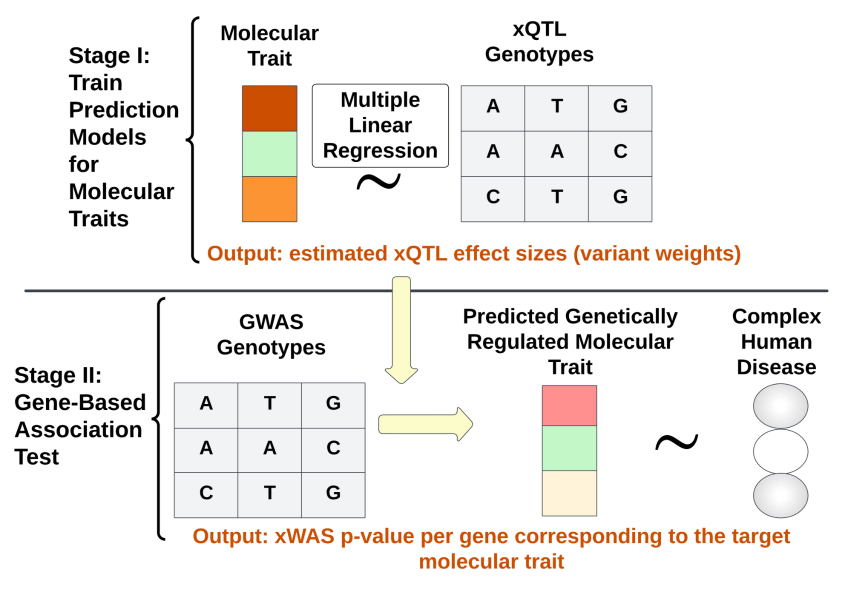
\includegraphics[width=0.7\textwidth]{../figs/xWAS.jpg}
  \end{figure}
  \begin{itemize}[<+(1)->]
    % \item TWAS combine transcriptomic + GWAS data
    % \item PWAS combine proteoomic + GWAS data \pause\pause

    \item TWAS/PWAS used to ID genes with \alert{genetically-regulated gene expression}/\alert{protein abundance} (\alert{GReX}/\alert{GReP}) associated with a phenotype \cite{barbeiraExploringPhenotypicConsequences2018, gusevTranscriptomewideAssociationStudy2019, strunzTranscriptomewideAssociationStudy2020,wingoIntegratingHumanBrain2021}

    % \item TWAS/PWAS risk genes have genetic effects potentially mediated through gene expression/protein abundance %$\rightarrow$ illustrate biological mechanisms of GWAS risk variants

    \item[$\rightarrow$\hspace{-1.5em}] \hspace{1em} illustrate biological mechanisms of GWAS risk variants
  \end{itemize}
% \includegraphics[width=0.75\textwidth]{../drawio_figs/bio_bg_2-xWAS1_1_4.drawio.pdf}
\note{xWAS to find candidate causal genes in candidate gene analysis following genomewide association studies\\[1em]
studies ofter lack transcriptomic/proteomic data}
\end{frame}




\begin{frame}{Standard Two-Stage xWAS\cite{gamazonGenebasedAssociationMethod2015, gusevIntegrativeApproachesLargescale2016, nagpalTIGARImprovedBayesian2019,huProteomewideAssociationStudies2025}} 

\Wider{
\begin{columns}
  \begin{column}[T]{.4\textwidth}
    \begin{figure}%
      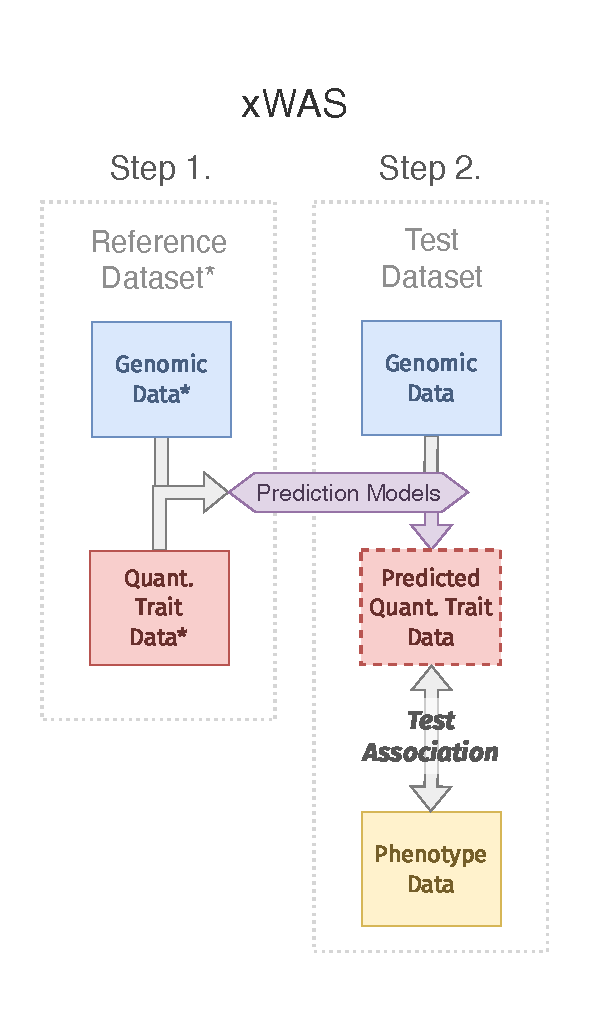
\includegraphics[trim={0 0 0 2cm},clip,width=14em]{../drawio_figs/bio_bg_2-Two_Step_xWAS_1.drawio.pdf}
    \end{figure}
  \end{column}
  %\hfill
  \begin{column}[T]{.6\textwidth}
    \vspace*{1em}
    \onslide<1->{{\large 1) Train models} \\}
    \onslide<2->{
    train quantitative trait prediction model from reference genotype, $\textbf{G}_0$, and quantitative trait (gene expression, protein abundance, etc.), $\textbf{Q}_0$, data from the same subjects\\[-0.5em]

    \[\textbf{Q}_0 = \textbf{G}_0 \textbf{w} + \boldsymbol{\epsilon}, \qquad \boldsymbol{\epsilon} \sim N(0,\, \sigma^2_{\epsilon}\textbf{I})\]

    where $\textbf{w}$ is xQTL weights\\[1em]
    }

    \onslide<3->{{\large 2) Test association}\\}
    \onslide<4->{
    test the association between predicted genetically-regulated quantitative trait (GReX or GReP) and phenotype of interest using estimated xQTL weights $\widehat{\textbf{w}}$

    \[\widehat{\textbf{GReX}} = \textbf{G}_{\text{test}} \widehat{\textbf{w}} \qquad \textnormal{(Individual-level)}\]}
  \end{column}
\end{columns}
}
\end{frame}



\section{BGW-xWAS Tool}



\begin{frame}{BGW-TWAS: Background}
  \begin{block}{BGW-TWAS Paper}
    Bayesian Genome-wide TWAS Method to Leverage both \textit{cis}- and \textit{trans}-eQTL Information through Summary Statistics. 2020. \textit{AJHG}. \url{https://pmc.ncbi.nlm.nih.gov/articles/PMC7536614/}.
  \end{block}
  \begin{itemize}[<+(1)->]
    \item BGW-TWAS\cite{luninghamBayesianGenomewideTWAS2020} tool originally developed for TWAS
    \item can be applied to other kinds of QTLs, not just eQTLs ("BGW-\textbf{x}WAS")
    \item \textbf{Motivation:}
    \begin{itemize}[<+->]
      \item existing TWAS methods only used \textit{cis}-SNPs (variants within $\pm$1MB of a gene) to fit GReX imputation models
      \item \textit{trans}-SNPs explain variation in expression quantitative traits, may be significant themselves
      \item[$\Rightarrow$] including \textit{trans}- variants expected to increase imputation accuracy of GReX and the power of TWASs
    \end{itemize}
    \item \textbf{Problem:} \only<+->{"the enormous computational cost required to fit \alert{20K GReX imputation models} for genomewide genes and \textbf{10M genotypes} \underline{per tissue type}"}
  \end{itemize}
\end{frame}


\begin{frame}[fragile]{BGW-xWAS Steps}

\onslide<1->{{\Large 1) Obtain Summary Statistics}\\
  generate single variant xQTL summary statistics (aka Score Statistics)
}

\onslide<2->{{\Large 2) Prune Genome Segments}\\
Select only the top \texttt{\$\{max\_blocks\}} (default: 50) \textit{trans}-genome blocks to use in joint-model training.

}

\onslide<3->{{\Large 3) Train Quantitative Trait Prediction Model}\\
  Train gene expression prediction model using single variant xQTL summary stats (obtained in Step 1) for genome blocks (obtained in Step 2)
}

\only<beamer>{\only<4>{{\Large 4) Predict Bayesian GReX/GReP/etc. (optional)}\\
 Predict GReX for test genotype data
}}

\onslide<5->{{\Large \st{4) Predict Bayesian GReX/GReP/etc. (optional)}}\\
 \st{Predict GReX for test genotype data}\\
 Used for individual-level test data only; later application instead uses summary-level test data.
}

\onslide<6->{{\Large 5) Association Studies}\\
  Perform using predicted GReX/GReP/etc. (obtained in Step 4) or using summary-level data from GWAS.
}

\end{frame}





\begin{frame}{BGW-xWAS: Model}
\Wider{
    \textbf{Bayesian variable selection regression (BVSR) with both \textit{cis}- and \textit{trans}-eQTLs:}
    \begin{align*}
     \onslide<2->{ \textbf{E}_g &= \textbf{G}_{\textit{cis}}\textbf{w}_{\!\textit{cis}} +  \textbf{G}_{\textit{trans}}\textbf{w}_{\!\textit{trans}} + \boldsymbol{\epsilon} \qquad\qquad\qquad\quad \epsilon_i\sim \N{0,\sigma_{\!\epsilon}^2} \\}
      \onslide<3->{w_{\!\textit{cis},i} &\sim \pi_{\!\textit{cis}} \, \N{0, \sigma^2_{\!\textit{cis}}\, \sigma_{\!\epsilon}^2} + (1-\pi_{\!\textit{cis}}) \; \partial_0(w_{\!\textit{cis},i}) \\}
      \onslide<4->{w_{\textit{trans},i} &\sim \pi_{\!\textit{trans}} \, \N{0, \sigma^2_{\!\textit{trans}}\, \sigma_{\!\epsilon}^2} + (1-\pi_{\!\textit{trans}}) \; \partial_0(w_{\textit{trans},i}) \\[-3em]}
      % \onslide<5->{\epsilon_i&\sim N(0,\sigma_{\!\epsilon}^2)\\[-4em]}
    \end{align*}
      \begin{itemize}[<+(4)->]
        \item xQTL effect size $w_{i}$ follows a "spike-and-slab" prior distribution–ie, we only retain a subset of the possible regressors
        % \item $\probs{w_{q,i}\sim N(0, \sigma_q^2\sigma_{\!\epsilon}^2)}=\pi_q$ \quad vs. \quad $\probs{w_{q,i}\sim \partial_0(w_{q,i})=0}=1-\pi_q$
        \item $\probs{w_{i}\sim \N{0, \sigma_{\!q}^2\sigma_{\!\epsilon}^2}}=\pi_q$ \quad vs. \quad $\probs{w_{i}=0}=1-\pi_q$,\quad\; $q\in \lbrace\textit{cis},\textit{trans} \rbrace$
        \item latent indicator vector $\boldsymbol{\gamma}_{p\times 1}$ is introduced to aid computation: $\gamma_i\sim\textnormal{Bern}(\pi_q)$%Each element $\gamma_{i}$ indicates whether $w_{i}=0$ ($\gamma_{i}=0$) or follows the $N(0,\sigma_{q}^2\sigma_{\!\epsilon}^2)$ distribution ($\gamma_{q,i}=1$).
        \item $\ex{\gamma_i}$ is the posterior probability ($\textnormal{PP}_i$) for the $i$th SNP to be an eQTL with non-zero effect size $w_{i}$.
      \end{itemize}    
}
\end{frame}



\begin{frame}[fragile]{BGW-xWAS: Model}
\Wider{
  \textbf{EM-MCMC Algorithm:}\\
  \onslide<2->{combines expectation–maximization (EM) algorithm with Markov Chain Monte Carlo (MCMC) algorithm\\[1em]}
    \begin{itemize}[<+(2)->]
      \item \textbf{E-step}: Use MCMC per genome block to estimate $(\textbf{w},\textbf{PP})$ from most recent estimation of $(\boldsymbol{\pi},\boldsymbol{\sigma}^2)$
      \item \textbf{M-step}: update $(\boldsymbol{\pi},\boldsymbol{\sigma}^2)$ using new estimates of $(\textbf{w},\textbf{PP})$ from E-step\\[1em]
    \end{itemize}
    \onslide<5->{Iterate until convergence,}\onslide<6->{ parallelize over genome blocks\\[2em]}

    \onslide<7->{\textbf{Final Estimate}:\quad $( \widehat{\textbf{w}}, \widehat{\textbf{PP}} )$
       \textbf{Predicted GReX/GReP/etc.}:\quad \[\widehat{\textbf{GReX}} = \sum_{i=1}^p \widetilde{G}_i(\widehat{PP_{i}}\,\widehat{w_{i}})\qquad \widetilde{\vec{G}}=\textnormal{\footnotesize test genotype data}\qquad \textnormal{(Individual-level xWAS)} \]}
}
\note{
  EM algorithm-iterative method to find (local) maximum likelihood or maximum a posteriori (MAP) estimates of parameters\\[2em]
  MCMC algorithms-used to draw samples from a probability distribution, used to study complex, high dimensional  probability distributions \\[2em]
  iterate until maximum a posteriori (MAPs) estimates converge (MAP is the mode of the posterior density.)\\[2em]
  }
\end{frame}


\begin{frame}[fragile]{BGW-TWAS: Summary-Level Association Test}
\onslide<+(1)->{GWAS summary statistics are often publicly available, and can be used to conduct summary-level association tests without the need for individual-level test genotype/phenotype data}

\onslide<+(1)->{%
Can use burden Z-score as implemented by S-PrediXcan\cite{barbeiraExploringPhenotypicConsequences2018}\\[0.5em]}

\onslide<+(1)->{  {\[{\widetilde{Z}_g} = \sum_{i \in \text{Model}} \frac{ (\widehat{PP_{i}}\,\widehat{w_{i}}) \; \widehat{\sigma_{i}}\; Z_{\textnormal{GWAS},i} }{ \sqrt{(\widehat{\vec{PP}}\,\widehat{\vec{w}})'\;\vec{V}\;(\widehat{\vec{PP}}\,\widehat{\vec{w}})} },\qquad\widehat{\sigma_{i}^{2}} = \text{Var}(\vec{G}_{0,i}),\qquad\vec{V} = \text{Cov}(\vec{G}_{0})\]}
}\vspace*{-1em}

\blfootnote{ \(\widehat{PP_{i}}\) estimated posterior causal probability for SNP \(i\)}
\blfootnote{ \(\widehat{w_{i}}\)\ estimated xQTL effect-size for SNP \(i\)}
\blfootnote{ \(Z_{\textnormal{GWAS},i}\)\ Z-score statistic values for single variant test (ie, GWAS)}
\blfootnote{ \(\widehat{\vec{PP}}\) estimated posterior causal probabilities from trained model}
\blfootnote{  \({\widehat{\vec{w}}}\)\ xQTL effect-sizes from trained model}\\
\blfootnote{ \(\vec{V}\)\ genotype covariance matrix (LD data) estimated from reference panel genotype data $\vec{G}_0$}
\blfootnote{ \(\vec{G}_{0}\)\ reference genotype matrix}
% \blfootnote{ \(\vec{G}_{0,i}\)\ genotype vector for SNP \(i\)}
\blfootnote{ \(\widehat{\sigma_{i}}\)\ estimated standard deviation of SNP \(i\) from genotype vector for SNP \(i\): \(\vec{G}_{0,i}\)}

\note{equivalent to FUSION if w hat is estimated using standardized reference data (which it is in BGW-TWAS);\\[2em]
Burden: A traditional test that aggregates the effects of variants within a gene.}
\end{frame}


\section{Application TWAS \& PWAS}

\subsection{Datasets}




\begin{frame}{Datasets}
  \begin{block}{Training Data: ROS/MAP\cite{bennettReligiousOrdersStudy2018}}
    Religious Orders Study and Rush Memory and Aging Project. 2018. \textit{
J. Alzheimer's Dis.}. \url{https://www.ncbi.nlm.nih.gov/pmc/articles/PMC6380522/}.
  \end{block}
% Dorsolateral prefrontal cortex (DLPFC) tissue data:
  % \onslide<2->{  %
  \begin{table}\footnotesize
    \begin{tabular}{llr}
      \toprule
      Dorsolateral prefrontal cortex (DLPFC) tissue data & N & Genes \\ \midrule
      RNA-Seq (Gene Expression) & 931 & 21,244 \\
      TMT Proteomics (Protein Abundance) & 716 & 12,175 \\
      \bottomrule
    \end{tabular}
  \end{table}
  % } %onslide

% \onslide<3->{ %
  \begin{block}{GWAS of Alzheimer's Disease\cite{bellenguezNewInsightsGenetic2022}}
    New insights into the genetic etiology of Alzheimer’s disease and related dementias. 2022. \textit{Nat. Genet.}. \url{https://www.nature.com/articles/s41588-022-01024-z}.
  \end{block}
  % } %onslide
  % \onslide<4->{ %
  \begin{itemize} %[<+->]
    \item 111,326 clinically diagnosed/"proxy" AD cases
    \item 677,663 controls
  \end{itemize}
  % } %onslide

\note{TMT Tandem mass tags;\\
ROS started in 1994, MAP started in 1997\\
longitudinal prospective clinical-pathologic cohort studies of aging and AD
}
\end{frame}



\subsection{Results}



\begin{frame}{Manhattan Plots}
  \hfill\\
  \Wider{
  \begin{figure}
    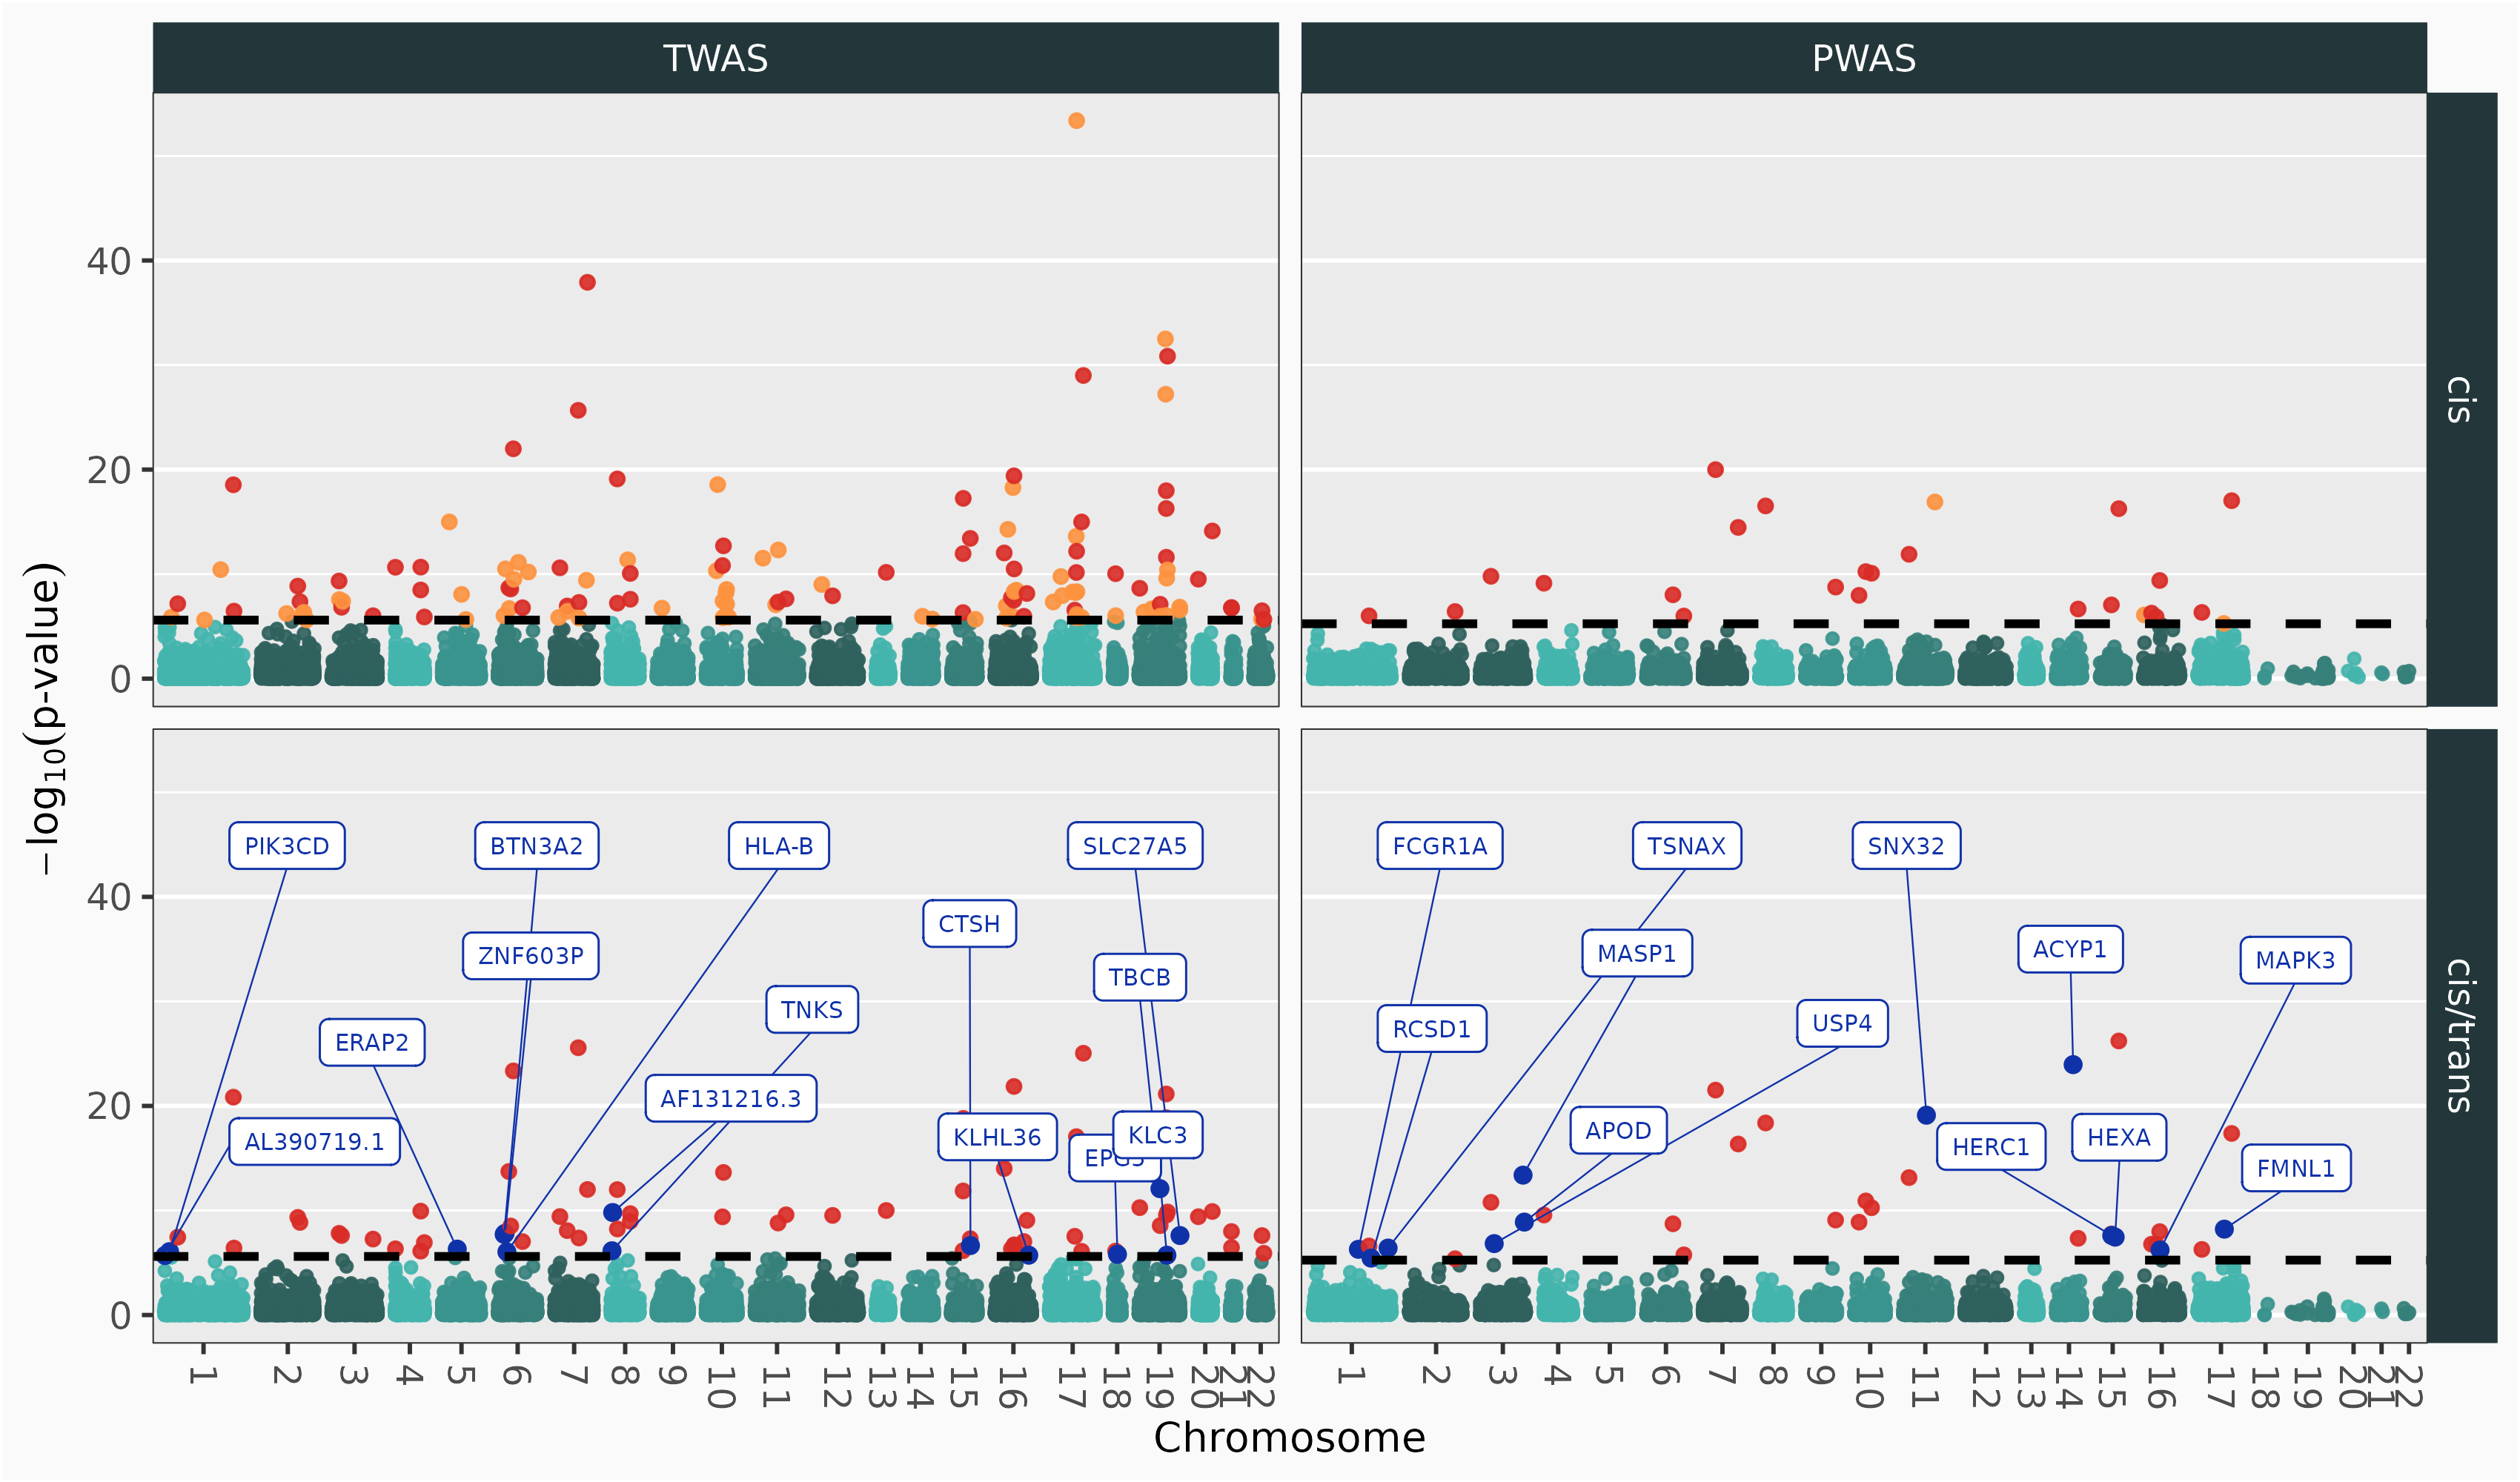
\includegraphics[width=\textwidth]{../figs/manplots_slides.png}
  \end{figure}}

  \note{
  orange genes ID'd by only cis model\\
  red genes ID'd both cis and cis/trans model\\
  blue labeled genes are ID'd only by cis/trans model\\
  EPG5 is hidden label }
\end{frame}




\begin{frame}{Results}
  \begin{table}\footnotesize
    \begin{tabular}{lrrrr}
      \toprule
       &  Total &   Significant &     NA &  \textit{trans}-only \\ \midrule
      cis-TWAS &  16408 &   130 &      305 &   - \\
      cis/trans-TWAS &  16676 &   74  &   555 &   298 \\[0.5em]
      cis-PWAS &  8829 &  25 &   1251 &  - \\
      cis/trans-PWAS &  8922 &  34  &  1293 &  84 \\
      \bottomrule
    \end{tabular}
  \end{table}    
  % \onslide<2->{
    \begin{figure}
      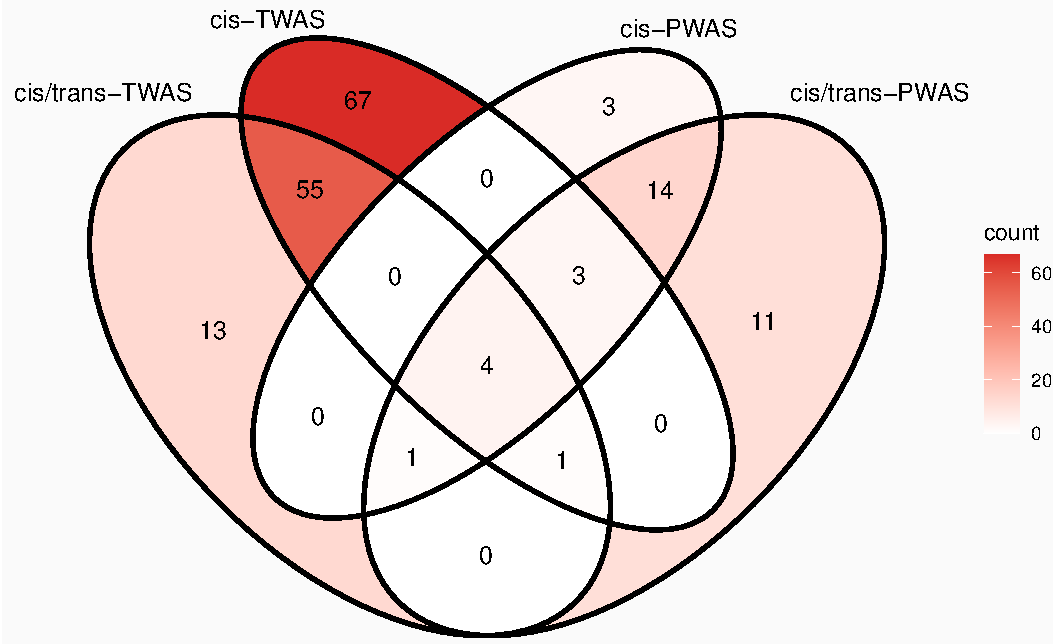
\includegraphics[width=0.65\textwidth]{../figs/venn-crop.pdf}\\
      \textbf{Overlap of Significant Risk Genes}
    \end{figure}
  % }
\note{
\begin{tabular}{lrrr}
 & prop\_sig & prop\_nonsig & prop\_NA \\\hline
cis-TWAS &  0.8\% & 97\% & 1.9\% \\
cis/trans-TWAS  & 0.4\% & 96\% & 3.3\% \\
cis-PWAS & 0.3\% & 86\% & 14\% \\
cis/trans-PWAS &  0.4\% & 85\% & 14\% \\
\end{tabular}
}
\end{frame}




\begin{frame}[fragile]{Results}
\Wider{
  \begin{table}\footnotesize
    \textbf{Risk Genes Identified by all xWAS}
    \begin{tabular}{lll}
      \toprule
       CHR &   Gene &  Function/Disease Association \\ \midrule
        7 & \textit{EGFR} & epidermal growth factor receptor \\
        8 & \textit{EPHX2} & lipid mediator; mutations associated with familial hypercholesterolemia \\
        15 & \textit{LACTB} & regulator of mitochondrial lipid metabolism \\
        17 & \textit{ACE} & angiotensin-converting enzyme \\
      \bottomrule
      % \multicolumn{3}{l}{\footnotesize $\ast$ previously-identified GWAS risk genes} \\
    \end{tabular}\\
  \end{table}
  % \onslide<2->{
  \begin{table}\footnotesize
  \textbf{Gene Ontology Pathway Enrichment Analysis (pathDIP}\cite{pastrelloPathDIP5Improving2024}\textbf{, PANTHER}\cite{miPANTHERPathwayOntologybased2009}\textbf{)}
    \begin{tabular}{lr}
      \toprule
      Enriched Paths Significant for all xWAS\\ \midrule
      \alert{Alzheimer disease-amyloid secretase}  \\
      EGF receptor signaling   \\
      Insulin/IGF pathway-mitogen activated protein kinase kinase/MAP kinase cascade   \\
      Interferon-gamma signaling   \\
      Ras Pathway   \\
      \bottomrule
    \end{tabular}
  \end{table}
  % }

}
\note<1->{ all are previously ID'd GWAS risk genes \\%}
  % \note<2>{ %
  PANTHER pathways, ontology-based pathway database\\
    * AD-amyloid secretase: disease pathway, enzymes that can cleave amyloid precursor protein\\
    * EGF receptor signaling: cell signaling/proliferation; issues w/ EGFR cancer, inflammation, impaired wound healing\\
     * Insulin/IGF ..: insulin receptor (IR), control cell fuel uptake/metabolism, defects insulin signaling involved in AD \\ %https://www-sciencedirect-com.proxy.library.emory.edu/science/article/pii/S0197458008001176
   * Interferon-gamma signaling: innate/adaptive immune system/intracell pathogens \\
    * Ras Pathway: respond to cell proliferation cues, oncogene 
    }
\end{frame}


\section{Summary}

\begin{frame}{Summary}
  \begin{itemize}[<+->]
    \item \textit{trans}-SNPs are important for explaining variation in expression quantitative traits, may be significant themselves
    \item traditional xWAS tools only incorporate \textit{cis}-SNPs
    \item BGW-xWAS tool accounts for both \textit{cis}- and \textit{trans}- variants
    \item BGW-xWAS uses various strategies make this computationally efficient: EM-MCMC, parallel computation, data pruning
     \item application study of AD xWAS identified risk genes previously identified in GWAS
    \item application study of AD xWAS show risk genes significantly enriched for AD-related pathways
    % \item \textit{cis}/\textit{trans}-xWAS able to identify 
  \end{itemize}
\end{frame}

\begin{frame}{Summary}
 \textbf{Limitations:}
\begin{itemize}[<+->]
      \item assumes a two-stage model for xWASs
      \item computational costs still substantial to train models for genome-wide genes per tissue type, per -omic data type:
      \item[\hspace*{2em}-] $\sim$30min of computation time per gene (in parallel with 4 CPU cores)
      \item PWAS based on protein abundance; does not consider effect of genetic variants on protein function\cite{brandesPWASProteomewideAssociation2020}
    \end{itemize}
\end{frame}


\section{References}
\setbeamertemplate{footline}{}
\begin{frame}[allowframebreaks,noframenumbering]%{References}
% \newgeometry{left=0.5cm, right=0.5cm, bottom=0.5cm, top=0.5cm}
\printbibliography[heading=none] 
\end{frame}


% \end{document}


